\documentclass[12pt]{article}

\usepackage{amsmath}
\usepackage{amssymb}
\usepackage{amsthm}
\usepackage{bm}
\usepackage{geometry}
\usepackage{amsmath}
\usepackage{amssymb}
\usepackage{amsthm}
\usepackage{tikz}
\usepackage{graphicx}
\usetikzlibrary{automata,positioning,arrows.meta}


\geometry{margin=1in}

\title{Assignment 2 Part A}
\author{Aarush Ram Anandh}
\date{\today}

\begin{document}
\maketitle
\subsection*{Problem 1}

For each training example \((x_i,y_i)\), define the indicator random variable

\[
Z_i^{(h)}
=
\mathbf{1}[h(x_i)\neq y_i]
\]

for a fixed hypothesis \(h \in \mathcal H\).

Since

\[
Z_i^{(h)} \in \{0,1\}
\]

we have

\[
0 \leq Z_i^{(h)} \leq 1
\]

Since the dataset is i.i.d., the random variables

\[
Z_1^{(h)}, Z_2^{(h)}, \dots, Z_m^{(h)}
\]

are independent.

Define the empirical error:

\[
\hat{\epsilon}(h)
=
\frac{1}{m}\sum_{i=1}^{m} Z_i^{(h)}
\]

Taking expectation,

\[
\mathbb E[\hat{\epsilon}(h)]
=
\mathbb E\left[
\frac{1}{m}\sum_{i=1}^{m} Z_i^{(h)}
\right]
\]

Using linearity of expectation,

\[
=
\frac{1}{m}\sum_{i=1}^{m}\mathbb E[Z_i^{(h)}]
\]

Since the samples are identically distributed,

\[
\mathbb E[Z_i^{(h)}]
=
\epsilon(h)
\]

where

\[
\epsilon(h)
=
P(h(x)\neq y)
\]

Therefore,

\[
\mathbb E[\hat{\epsilon}(h)]
=
\frac{1}{m}\sum_{i=1}^{m}\epsilon(h)
=
\epsilon(h)
\]

Hence, the empirical error is the sample mean of bounded independent random variables whose expectation equals the true error.

\paragraph{Hoeffding's Inequality}

For independent random variables bounded in \([0,1]\),

\[
P\left(
\left|
\frac{1}{m}\sum_{i=1}^{m} Z_i^{(h)}
-
\mathbb E\left[
\frac{1}{m}\sum_{i=1}^{m} Z_i^{(h)}
\right]
\right|
>
\gamma
\right)
\leq
2e^{-2m\gamma^2}
\]

Substituting the expectation,

\[
P\left(
|\hat{\epsilon}(h)-\epsilon(h)|
>
\gamma
\right)
\leq
2e^{-2m\gamma^2}
\]

This bound holds for a fixed hypothesis \(h\).

Define the bad event

\[
A_h
=
\{
|\hat{\epsilon}(h)-\epsilon(h)|
>
\gamma
\}
\]

The event that at least one hypothesis fails is

\[
\bigcup_{h\in\mathcal H} A_h
\]

Using the union bound,

\[
P\left(
\bigcup_{h\in\mathcal H} A_h
\right)
\leq
\sum_{h\in\mathcal H} P(A_h)
\]

From Hoeffding's inequality,

\[
P(A_h)
\leq
2e^{-2m\gamma^2}
\]

for every \(h\in\mathcal H\).

Since \(|\mathcal H|=k\),

\[
\sum_{h\in\mathcal H} P(A_h)
\leq
k \cdot 2e^{-2m\gamma^2}
\]

Hence,

\[
P\left(
\exists h\in\mathcal H :
|\hat{\epsilon}(h)-\epsilon(h)|
>
\gamma
\right)
\leq
2k e^{-2m\gamma^2}
\]

The complementary event is

\[
\forall h\in\mathcal H :
|\hat{\epsilon}(h)-\epsilon(h)|
\leq
\gamma
\]

Therefore,

\[
P\left(
\forall h\in\mathcal H :
|\hat{\epsilon}(h)-\epsilon(h)|
\leq
\gamma
\right)
=
1-
P\left(
\exists h\in\mathcal H :
|\hat{\epsilon}(h)-\epsilon(h)|
>
\gamma
\right)
\]

Using the previous bound,

\[
\geq
1-2k e^{-2m\gamma^2}
\]

We require this probability to be at least \(1-\delta\). Hence it is sufficient that

\[
1-2k e^{-2m\gamma^2}
\geq
1-\delta
\]

Rearranging,

\[
2k e^{-2m\gamma^2}
\leq
\delta
\]

Divide by \(2k\):

\[
e^{-2m\gamma^2}
\leq
\frac{\delta}{2k}
\]

Take logarithms:

\[
-2m\gamma^2
\leq
\log\left(\frac{\delta}{2k}\right)
\]

Multiply by \(-1\), reversing the inequality:

\[
2m\gamma^2
\geq
\log\left(\frac{2k}{\delta}\right)
\]

Finally,

\[
m
\geq
\frac{1}{2\gamma^2}
\log\left(\frac{2k}{\delta}\right)
\]

Thus, the required sample complexity bound is proved.
This establishes a uniform deviation guarantee over the hypothesis class.
\subsection*{Question 2}

Let the centered dataset be

\[
X \in \mathbb R^{n\times d}
\]

with rows \(x_1,x_2,\dots,x_n\), and

\[
\frac1n\sum_{i=1}^n x_i = 0
\]

Define the sample covariance matrix

\[
\Sigma = \frac1n X^TX
\]

We proceed from first principles.

\subsubsection*{Part 1}

We want the variance of the data after projection onto a unit vector \(v\).

Each projected point is

\[
z_i = x_i^T v
\]

Since the data is centered,

\[
\frac1n\sum_{i=1}^n z_i
=
\frac1n\sum_{i=1}^n x_i^Tv
=
\left(
\frac1n\sum_{i=1}^n x_i
\right)^T v
=
0
\]

Therefore the variance of the projected data is

\[
\mathrm{Var}(z)
=
\frac1n\sum_{i=1}^n z_i^2
\]

Substitute \(z_i=x_i^Tv\):

\[
=
\frac1n\sum_{i=1}^n (x_i^Tv)^2
\]

Using

\[
(x_i^Tv)^2
=
v^Tx_i x_i^T v
\]

we obtain

\[
\mathrm{Var}(z)
=
\frac1n\sum_{i=1}^n v^Tx_i x_i^Tv
\]

Since \(v\) does not depend on \(i\),

\[
=
v^T
\left(
\frac1n\sum_{i=1}^n x_i x_i^T
\right)
v
\]

But

\[
\frac1n\sum_{i=1}^n x_i x_i^T
=
\frac1n X^TX
=
\Sigma
\]

Therefore,

\[
\mathrm{Var}(z)
=
v^T\Sigma v
\]

Thus maximizing projected variance is equivalent to maximizing

\[
v^T\Sigma v
\]

subject to

\[
\|v\|_2=1
\]

\subsubsection*{Part 2}

The optimization problem is

\[
\max_v v^T\Sigma v
\]

subject to

\[
v^Tv=1
\]

Introduce a Lagrange multiplier \(\lambda\).

Define the Lagrangian:

\[
\mathcal L(v,\lambda)
=
v^T\Sigma v
-
\lambda(v^Tv-1)
\]

Take gradient with respect to \(v\):

\[
\nabla_v \mathcal L
=
2\Sigma v - 2\lambda v
\]

Set gradient equal to zero:

\[
2\Sigma v - 2\lambda v = 0
\]

Dividing by \(2\),

\[
\Sigma v = \lambda v
\]

This is precisely the eigenvalue equation.

Therefore the optimal direction \(v\) must be an eigenvector of \(\Sigma\).

Now evaluate the objective:

\[
v^T\Sigma v
=
v^T(\lambda v)
=
\lambda v^Tv
\]

Since \(v^Tv=1\),

\[
v^T\Sigma v = \lambda
\]

Hence maximizing variance means choosing the eigenvector corresponding to the largest eigenvalue.

That eigenvector is the first principal component.

\subsubsection*{Part 3}

Consider the dataset

\[
(1,1), (2,2), (3,2), (4,3)
\]

\paragraph{Step 1: Compute the mean}

\[
\mu
=
\left(
\frac{1+2+3+4}{4},
\frac{1+2+2+3}{4}
\right)
=
(2.5,2)
\]

\paragraph{Step 2: Center the data}

\[
X=
\begin{bmatrix}
-1.5 & -1 \\
-0.5 & 0 \\
0.5 & 0 \\
1.5 & 1
\end{bmatrix}
\]

\paragraph{Step 3: Compute covariance matrix}

\[
X^TX
=
\begin{bmatrix}
5 & 3 \\
3 & 2
\end{bmatrix}
\]

Therefore

\[
\Sigma
=
\frac14
\begin{bmatrix}
5 & 3 \\
3 & 2
\end{bmatrix}
=
\begin{bmatrix}
1.25 & 0.75 \\
0.75 & 0.5
\end{bmatrix}
\]

\paragraph{Step 4: Find eigenvalues}

Solve

\[
\det(\Sigma-\lambda I)=0
\]

\[
\begin{vmatrix}
1.25-\lambda & 0.75 \\
0.75 & 0.5-\lambda
\end{vmatrix}
=0
\]

Expanding,

\[
(1.25-\lambda)(0.5-\lambda)-0.75^2=0
\]

\[
\lambda^2 -1.75\lambda +0.0625 =0
\]

The eigenvalues are

\[
\lambda_1 \approx 1.7135
\]

and

\[
\lambda_2 \approx 0.0365
\]

The principal eigenvalue is

\[
\lambda_1 \approx 1.7135
\]

\paragraph{Step 5: Find principal eigenvector}

Solving

\[
(\Sigma-\lambda_1 I)v=0
\]

gives approximately

\[
v=
\begin{bmatrix}
0.851 \\
0.526
\end{bmatrix}
\]

This is the direction of maximum variance.

\paragraph{Step 6: Compute projections}

Projection scalars:

\[
z_i = x_i^T v
\]

For the centered points:

\[
(-1.5,-1)\to -1.8025
\]

\[
(-0.5,0)\to -0.4255
\]

\[
(0.5,0)\to 0.4255
\]

\[
(1.5,1)\to 1.8025
\]

The projected vectors are

\[
z_i v
\]

which place every point onto the principal component line.

\paragraph{Step 7: Plots}

\begin{figure}[h]
\centering
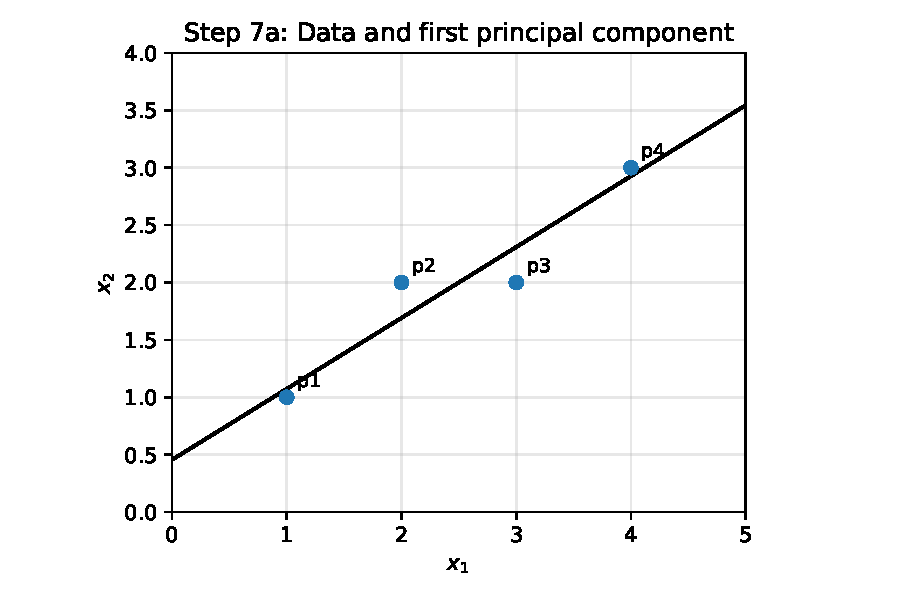
\includegraphics[width=0.7\linewidth]{figures/pca_data_line.pdf}
\caption{Step 7a: Data points and the first principal component line.}
\end{figure}

\begin{figure}[h]
\centering
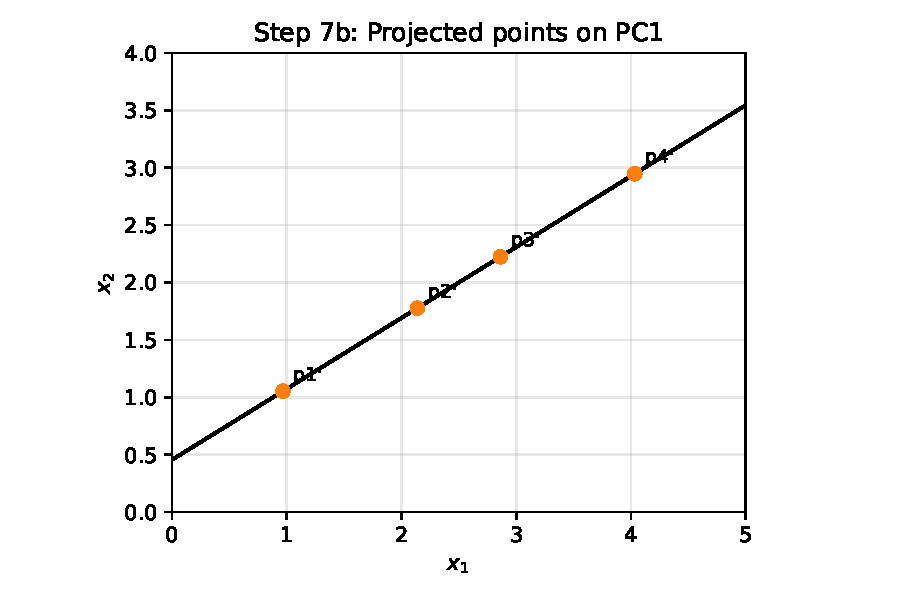
\includegraphics[width=0.7\linewidth]{figures/pca_projected.pdf}
\caption{Step 7b: Projected points on the first principal component.}
\end{figure}

Geometrically, this means the data are best summarized by a line through the mean in the direction of maximum variance.

\subsection*{Problem 3}

Let \(x\) denote the observed variable and \(z\) denote a latent variable.
Assume the model defines a joint distribution

\[
p(x,z)
\]

The marginal likelihood of the observed data is

\[
p(x)
=
\int p(x,z)\,dz
\]

and therefore the log-likelihood is

\[
\log p(x)
=
\log \int p(x,z)\,dz
\]

The quantity \(\log p(x)\) is generally difficult to optimize directly because the integral over the latent variable \(z\) is often intractable.

To obtain a tractable lower bound, introduce an auxiliary distribution

\[
q(z)
\]

such that

\[
q(z) > 0
\]

whenever

\[
p(x,z) > 0
\]

We now rewrite the marginal likelihood by multiplying and dividing by \(q(z)\):

\[
\log p(x)
=
\log \int p(x,z)\frac{q(z)}{q(z)}\,dz
\]

Rearranging,

\[
=
\log \int q(z)\frac{p(x,z)}{q(z)}\,dz
\]

Using expectation notation,

\[
=
\log \mathbb E_{z\sim q}
\left[
\frac{p(x,z)}{q(z)}
\right]
\]

At this point we apply Jensen's inequality.

Since the logarithm is concave,

\[
\log \mathbb E[Y]
\geq
\mathbb E[\log Y]
\]

for any positive random variable \(Y\).

Let

\[
Y
=
\frac{p(x,z)}{q(z)}
\]

Then,

\[
\log \mathbb E_{z\sim q}
\left[
\frac{p(x,z)}{q(z)}
\right]
\geq
\mathbb E_{z\sim q}
\left[
\log \frac{p(x,z)}{q(z)}
\right]
\]

Therefore,

\[
\log p(x)
\geq
\mathbb E_{z\sim q}
\left[
\log \frac{p(x,z)}{q(z)}
\right]
\]

Define the Evidence Lower Bound (ELBO):

\[
\mathrm{ELBO}(q)
:=
\mathbb E_{z\sim q}
\left[
\log \frac{p(x,z)}{q(z)}
\right]
\]

Hence,

\[
\boxed{
\log p(x)
\geq
\mathrm{ELBO}(q)
}
\]

which proves that the ELBO is a lower bound on the data log-likelihood.

\subsubsection*{Gap Between the Evidence and the ELBO}

Consider the Kullback-Leibler divergence between the auxiliary distribution \(q(z)\) and the posterior distribution \(p(z|x)\):

\[
\mathrm{KL}(q(z)\|p(z|x))
=
\mathbb E_{z\sim q}
\left[
\log \frac{q(z)}{p(z|x)}
\right]
\]

Using Bayes' rule,

\[
p(z|x)
=
\frac{p(x,z)}{p(x)}
\]

Substituting into the KL divergence,

\[
=
\mathbb E_{z\sim q}
\left[
\log
\frac{q(z)p(x)}{p(x,z)}
\right]
\]

Using logarithm identities,

\[
=
\mathbb E_{z\sim q}
\left[
\log q(z)
+
\log p(x)
-
\log p(x,z)
\right]
\]

Since \(\log p(x)\) does not depend on \(z\),

\[
=
\log p(x)
+
\mathbb E_{z\sim q}[\log q(z)]
-
\mathbb E_{z\sim q}[\log p(x,z)]
\]

Rearranging,

\[
=
\log p(x)
-
\mathbb E_{z\sim q}
\left[
\log \frac{p(x,z)}{q(z)}
\right]
\]

Using the definition of the ELBO,

\[
\boxed{
\mathrm{KL}(q(z)\|p(z|x))
=
\log p(x)
-
\mathrm{ELBO}(q)
}
\]

\paragraph{ELBO identity.}
\[
\log p(x)
=
\mathrm{ELBO}(q)
+
\mathrm{KL}(q(z)\|p(z|x))
\]

Since KL divergence is always nonnegative,

\[
\mathrm{KL}(q(z)\|p(z|x))
\geq 0
\]

it follows that

\[
\mathrm{ELBO}(q)
\leq
\log p(x)
\]

Thus the ELBO is indeed a lower bound on the evidence.

\subsubsection*{Reconstruction and Regularization Form}

We now expand the ELBO into interpretable terms.

Using the factorization

\[
p(x,z)
=
p(x|z)p(z)
\]

the ELBO becomes

\[
\mathrm{ELBO}(q)
=
\mathbb E_{z\sim q}
\left[
\log
\frac{p(x|z)p(z)}{q(z)}
\right]
\]

Using logarithm properties,

\[
=
\mathbb E_{z\sim q}[\log p(x|z)]
+
\mathbb E_{z\sim q}
\left[
\log \frac{p(z)}{q(z)}
\right]
\]

Rewrite the second term:

\[
=
\mathbb E_{z\sim q}[\log p(x|z)]
-
\mathbb E_{z\sim q}
\left[
\log \frac{q(z)}{p(z)}
\right]
\]

Recognize the KL divergence:

\[
\boxed{
\mathrm{ELBO}(q)
=
\mathbb E_{z\sim q}[\log p(x|z)]
-
\mathrm{KL}(q(z)\|p(z))
}
\]

Therefore maximizing the ELBO is equivalent to:

\[
\boxed{
\max \mathrm{ELBO}(q)
}
\]

or equivalently minimizing

\[
\boxed{
-\mathrm{ELBO}(q)
=
-
\mathbb E_{z\sim q}[\log p(x|z)]
+
\mathrm{KL}(q(z)\|p(z))
}
\]

The two terms have the following interpretations:

\paragraph{1. Reconstruction Term}

\[
\mathbb E_{z\sim q}[\log p(x|z)]
\]

This term measures how well the latent variable \(z\) can reconstruct or explain the observed data \(x\).
Maximizing this term improves reconstruction quality.

\paragraph{2. KL-Regularization Term}

\[
\mathrm{KL}(q(z)\|p(z))
\]

This term measures how far the auxiliary distribution \(q(z)\) is from the prior distribution \(p(z)\).
Minimizing this term regularizes the latent representation and prevents the latent distribution from deviating excessively from the prior.

Hence the ELBO simultaneously balances:

\[
\text{data reconstruction}
\quad \text{and} \quad
\text{latent regularization}
\]

which forms the foundation of variational inference and variational autoencoders.

\subsection*{Problem 4}

Consider the input sequence

\[
s = w_1,w_2,\dots,w_n
\]

A decoder-only Transformer maps this sequence to output embeddings

\[
O = [o_1,o_2,\dots,o_n]
\]

For any prefix

\[
s_i = w_1,w_2,\dots,w_i
\]

let the corresponding output sequence be

\[
O_i = [o_1,o_2,\dots,o_i]
\]

We must prove that in a decoder-only Transformer,

\[
s_i = w_1,\dots,w_i
\quad \Longrightarrow \quad
O_i = [o_1,\dots,o_i]
\]

That is, the output representation at position \(i\) depends only on the prefix up to position \(i\), and not on future tokens.

\subsubsection*{Decoder-Only Transformer Structure}

A decoder-only Transformer uses \textbf{causal masked self-attention}.

For a sequence of embeddings

\[
X = [x_1,x_2,\dots,x_n]
\]

the model computes:

\[
Q = XW_Q,
\qquad
K = XW_K,
\qquad
V = XW_V
\]

where:

\[
Q \in \mathbb R^{n\times d_k},
\qquad
K \in \mathbb R^{n\times d_k},
\qquad
V \in \mathbb R^{n\times d_v}
\]

The attention score matrix is

\[
A
=
\frac{QK^T}{\sqrt{d_k}}
\]

The decoder applies a causal mask \(M\):

\[
M_{ij}
=
\begin{cases}
0 & j \leq i \\
-\infty & j > i
\end{cases}
\]

Thus the masked attention becomes

\[
\widetilde A
=
A + M
\]

and the attention weights are

\[
P
=
\mathrm{softmax}(\widetilde A)
\]

Finally the outputs are

\[
O = PV
\]

\subsubsection*{Causal Structure}

The mask forces

\[
P_{ij}=0
\quad \text{whenever } j>i
\]

because

\[
e^{-\infty}=0
\]

Therefore,

\[
o_i
=
\sum_{j=1}^n P_{ij}v_j
\]

reduces to

\[
o_i
=
\sum_{j=1}^i P_{ij}v_j
\]

Hence the output at position \(i\) depends only on

\[
v_1,v_2,\dots,v_i
\]

which themselves depend only on

\[
w_1,w_2,\dots,w_i
\]

Therefore,

\[
o_i
=
f(w_1,\dots,w_i)
\]

for some function \(f\).

Thus future tokens

\[
w_{i+1},\dots,w_n
\]

cannot influence \(o_i\).

Hence,

\[
s_i = w_1,\dots,w_i
\Longrightarrow
O_i=[o_1,\dots,o_i]
\]

which proves the required property.

\subsubsection*{Proof by Mathematical Implication}

We now formalize the argument.

Assume:

\[
j>i
\]

By definition of the causal mask,

\[
M_{ij}=-\infty
\]

Therefore,

\[
\widetilde A_{ij}
=
A_{ij}+M_{ij}
=
-\infty
\]

Applying softmax,

\[
P_{ij}
=
\frac{e^{\widetilde A_{ij}}}
{\sum_{k=1}^n e^{\widetilde A_{ik}}}
=
0
\]

Hence:

\[
j>i
\Longrightarrow
P_{ij}=0
\]

Now,

\[
o_i
=
\sum_{j=1}^n P_{ij}v_j
\]

Using the implication above,

\[
=
\sum_{j=1}^i P_{ij}v_j
\]

Thus:

\[
o_i
\text{ is independent of }
v_{i+1},\dots,v_n
\]

Since each \(v_j\) is computed from token \(w_j\),

\[
o_i
\text{ is independent of }
w_{i+1},\dots,w_n
\]

Therefore:

\[
o_i
=
f(w_1,\dots,w_i)
\]

for every \(i\).

Consequently,

\[
O_i=[o_1,\dots,o_i]
\]

depends only on the prefix

\[
s_i=w_1,\dots,w_i
\]

which proves causality.

\subsubsection*{Matrix Interpretation}

The causal attention matrix has the form

\[
P
=
\begin{bmatrix}
\ast & 0 & 0 & 0 & \cdots \\
\ast & \ast & 0 & 0 & \cdots \\
\ast & \ast & \ast & 0 & \cdots \\
\ast & \ast & \ast & \ast & \cdots \\
\vdots & \vdots & \vdots & \vdots & \ddots
\end{bmatrix}
\]

where:

\[
\ast \neq 0
\]

Only lower-triangular entries may be nonzero.

Therefore position \(i\) can attend only to positions

\[
1,\dots,i
\]

and never to future positions.

\subsubsection*{Flow of Information}

\[
w_1 \rightarrow o_1
\]

\[
w_1,w_2 \rightarrow o_2
\]

\[
w_1,w_2,w_3 \rightarrow o_3
\]

\[
\vdots
\]

\[
w_1,\dots,w_i \rightarrow o_i
\]

but never

\[
w_{i+1}\rightarrow o_i
\]

This directional flow is enforced entirely by the causal mask.

\subsubsection*{Importance in Autoregressive Language Modeling}

Autoregressive language models factorize the joint probability as

\[
p(w_1,\dots,w_n)
=
\prod_{i=1}^n p(w_i|w_1,\dots,w_{i-1})
\]

Therefore prediction at position \(i\) must depend only on previous tokens.

If future tokens were visible during training, the model could trivially copy future information, causing information leakage.

The causal mask prevents this leakage and guarantees that:

\[
o_i
\text{ contains only past context}
\]

Thus training and inference follow the same probabilistic structure.

This property is essential because it ensures:

\[
\text{training objective}
=
\text{generation objective}
\]

which allows decoder-only Transformers such as GPT models to generate text autoregressively one token at a time.
This prefix-consistency property is what makes next-token training well-defined and prevents leakage from future tokens.



\subsection*{Problem 5}

We model the system as a Markov Decision Process (MDP).

\subsubsection*{MDP Definition}

An MDP is defined by:

\[
(\mathcal S,\mathcal A,P,R,\gamma)
\]

where:

\[
\mathcal S = \{I,O\}
\]

with:

\[
I = \text{Idle state}
\]

\[
O = \text{Occupied state}
\]

The action space is

\[
\mathcal A = \{\text{stay},\text{switch}\}
\]

The rewards are state-dependent:

\[
R(I) = -3
\]

\[
R(O) = +1
\]

The discount factor satisfies

\[
0<\gamma<1
\]

The system is noisy.

With probability

\[
1-\epsilon
\]

the intended action occurs, and with probability

\[
\epsilon
\]

the opposite transition occurs.

\subsubsection*{Transition Dynamics}

If the action is \(\text{stay}\):

\[
P(I|I,\text{stay}) = 1-\epsilon
\]

\[
P(O|I,\text{stay}) = \epsilon
\]

\[
P(O|O,\text{stay}) = 1-\epsilon
\]

\[
P(I|O,\text{stay}) = \epsilon
\]

If the action is \(\text{switch}\):

\[
P(O|I,\text{switch}) = 1-\epsilon
\]

\[
P(I|I,\text{switch}) = \epsilon
\]

\[
P(I|O,\text{switch}) = 1-\epsilon
\]

\[
P(O|O,\text{switch}) = \epsilon
\]

\subsubsection*{MDP Transition Diagram}

\begin{center}

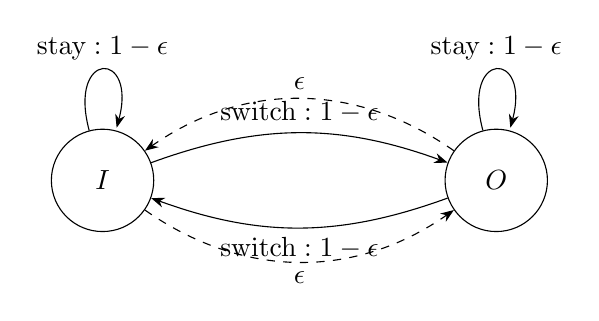
\begin{tikzpicture}[
    >=Stealth,
    node distance=5cm,
    every state/.style={draw,minimum size=1.3cm}
]

\node[state] (I) {$I$};
\node[state,right of=I] (O) {$O$};

\draw[->,bend left=20]
(I) to
node[above]
{\(\text{switch}:1-\epsilon\)}
(O);

\draw[->,bend left=20]
(O) to
node[below]
{\(\text{switch}:1-\epsilon\)}
(I);

\draw[->]
(I) edge[loop above]
node
{\(\text{stay}:1-\epsilon\)}
(I);

\draw[->]
(O) edge[loop above]
node
{\(\text{stay}:1-\epsilon\)}
(O);

\draw[->,dashed,bend right=35]
(I) to
node[below]
{\(\epsilon\)}
(O);

\draw[->,dashed,bend right=35]
(O) to
node[above]
{\(\epsilon\)}
(I);

\end{tikzpicture}

\end{center}

The dashed transitions represent failures caused by system noise.

% ---------------------------------------------------
% Optimal Policy
% ---------------------------------------------------

\subsubsection*{Optimal Policy}

We now determine the optimal policy.

The occupied state yields reward

\[
+1
\]

while the idle state yields reward

\[
-3
\]

Therefore the objective is to maximize the long-term probability of being in state \(O\).

Suppose we are in state \(I\).

If we choose \(\text{stay}\),

\[
P(O|I,\text{stay})=\epsilon
\]

If we choose \(\text{switch}\),

\[
P(O|I,\text{switch})=1-\epsilon
\]

Since

\[
0<\epsilon<\frac12
\]

we have

\[
1-\epsilon > \epsilon
\]

Hence:

\[
P(O|I,\text{switch})
>
P(O|I,\text{stay})
\]

Therefore switching is strictly better in state \(I\).

Now suppose we are in state \(O\).

If we choose \(\text{stay}\),

\[
P(O|O,\text{stay})=1-\epsilon
\]

If we choose \(\text{switch}\),

\[
P(O|O,\text{switch})=\epsilon
\]

Again,

\[
1-\epsilon>\epsilon
\]

Hence:

\[
P(O|O,\text{stay})
>
P(O|O,\text{switch})
\]

Therefore staying is strictly better in state \(O\).

Thus the optimal policy is

\[
\boxed{
\pi^\ast(I)=\text{switch}
}
\]

\[
\boxed{
\pi^\ast(O)=\text{stay}
}
\]

Intuitively:

\[
\text{Move toward } O
\quad\text{and remain there.}
\]

% ---------------------------------------------------
% Value Function
% ---------------------------------------------------

\subsubsection*{Value Function Under the Optimal Policy}

Let

\[
V^\ast(I)
\]

and

\[
V^\ast(O)
\]

denote the optimal value functions.

Using the Bellman equations:

\[
V^\ast(I)
=
-3
+
\gamma
\left[
(1-\epsilon)V^\ast(O)
+
\epsilon V^\ast(I)
\right]
\]

since under the optimal policy we switch from \(I\).

Similarly,

\[
V^\ast(O)
=
1
+
\gamma
\left[
(1-\epsilon)V^\ast(O)
+
\epsilon V^\ast(I)
\right]
\]

since under the optimal policy we stay in \(O\).

Define

\[
X
=
(1-\epsilon)V^\ast(O)
+
\epsilon V^\ast(I)
\]

Then:

\[
V^\ast(I)=-3+\gamma X
\]

\[
V^\ast(O)=1+\gamma X
\]

Substitute into \(X\):

\[
X
=
(1-\epsilon)(1+\gamma X)
+
\epsilon(-3+\gamma X)
\]

Expand:

\[
=
1-\epsilon+\gamma(1-\epsilon)X
-3\epsilon+\gamma\epsilon X
\]

Combine terms:

\[
X
=
1-4\epsilon+\gamma X
\]

Therefore,

\[
X-\gamma X
=
1-4\epsilon
\]

\[
(1-\gamma)X
=
1-4\epsilon
\]

Hence,

\[
X
=
\frac{1-4\epsilon}{1-\gamma}
\]

Substitute back:

\[
V^\ast(I)
=
-3
+
\gamma
\frac{1-4\epsilon}{1-\gamma}
\]

Therefore,

\[
\boxed{
V^\ast(I)
=
-3
+
\frac{\gamma(1-4\epsilon)}{1-\gamma}
}
\]

Similarly,

\[
V^\ast(O)
=
1
+
\gamma
\frac{1-4\epsilon}{1-\gamma}
\]

Thus,

\[
\boxed{
V^\ast(O)
=
1
+
\frac{\gamma(1-4\epsilon)}{1-\gamma}
}
\]

These are the optimal discounted infinite-horizon values for the MDP.
Sanity check: since $V^\ast(O)=V^\ast(I)+4$, the occupied state is always more valuable than the idle state.
\end{document}